% !TeX program = xelatex
\documentclass[12pt, a4paper]{article}
\usepackage{amsmath}
\usepackage{xeCJK}
\usepackage{amsmath}
\usepackage{amssymb}
\usepackage{parskip}
\usepackage{tikz}
\usepackage{enumitem}

\setmainfont{Latin Modern Roman}
\setCJKmainfont{Noto Serif CJK TC}

\title{Electrostatic field}

\begin{document}
\section*{Electric potential}
Curl-free vector field
$$
\textbf{E} = -\nabla V
$$
Physical meaning: \\
\textbf{Work: } a charge $P_1 \to P_2$, and unit charge against $\vec E$ from $P_1 \to P_2$
\begin{center}
	

\tikzset{every picture/.style={line width=0.75pt}} %set default line width to 0.75pt        

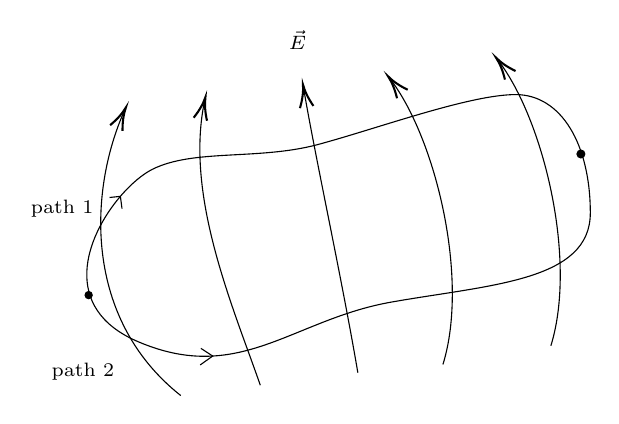
\begin{tikzpicture}[x=0.75pt,y=0.75pt,yscale=-1,xscale=1]
%uncomment if require: \path (0,300); %set diagram left start at 0, and has height of 300

%Shape: Polygon Curved [id:ds6671658677765401] 
\draw   (219.43,130.79) .. controls (239.43,120.79) and (270.71,126.56) .. (299.43,118.79) .. controls (328.15,111.03) and (372.43,94.79) .. (394.43,94.79) .. controls (416.43,94.79) and (430.43,118.79) .. (430.43,151.79) .. controls (430.43,184.79) and (382.11,186.35) .. (334.43,194.79) .. controls (299.89,200.91) and (277.08,219.15) .. (248.51,220.76) .. controls (237.64,221.38) and (225.93,219.58) .. (212.43,213.79) .. controls (174.91,197.72) and (187.22,163.47) .. (204.02,143.81) .. controls (209.17,137.79) and (214.74,133.14) .. (219.43,130.79) -- cycle ;
%Curve Lines [id:da19358608924661447] 
\draw    (233.09,239.79) .. controls (185.81,202.36) and (188.98,140.68) .. (205.89,102.72) ;
\draw [shift={(206.67,101)}, rotate = 114.94] [color={rgb, 255:red, 0; green, 0; blue, 0 }  ][line width=0.75]    (10.93,-3.29) .. controls (6.95,-1.4) and (3.31,-0.3) .. (0,0) .. controls (3.31,0.3) and (6.95,1.4) .. (10.93,3.29)   ;
%Curve Lines [id:da7659480223177946] 
\draw    (271.43,234.79) .. controls (257.57,195.19) and (234.89,142.85) .. (244.69,97.38) ;
\draw [shift={(245,96)}, rotate = 103] [color={rgb, 255:red, 0; green, 0; blue, 0 }  ][line width=0.75]    (10.93,-3.29) .. controls (6.95,-1.4) and (3.31,-0.3) .. (0,0) .. controls (3.31,0.3) and (6.95,1.4) .. (10.93,3.29)   ;
%Curve Lines [id:da09978817632588866] 
\draw    (318.43,228.79) .. controls (310.55,182.5) and (297.82,124.56) .. (292.25,91.49) ;
\draw [shift={(292,90)}, rotate = 80.6] [color={rgb, 255:red, 0; green, 0; blue, 0 }  ][line width=0.75]    (10.93,-3.29) .. controls (6.95,-1.4) and (3.31,-0.3) .. (0,0) .. controls (3.31,0.3) and (6.95,1.4) .. (10.93,3.29)   ;
%Curve Lines [id:da24731738696531214] 
\draw    (359.43,224.79) .. controls (372.23,183.42) and (355.93,115.86) .. (334.01,87.28) ;
\draw [shift={(333,86)}, rotate = 51.1] [color={rgb, 255:red, 0; green, 0; blue, 0 }  ][line width=0.75]    (10.93,-3.29) .. controls (6.95,-1.4) and (3.31,-0.3) .. (0,0) .. controls (3.31,0.3) and (6.95,1.4) .. (10.93,3.29)   ;
%Curve Lines [id:da513203566352172] 
\draw    (411.43,215.79) .. controls (424.23,174.42) and (407.93,106.86) .. (386.01,78.28) ;
\draw [shift={(385,77)}, rotate = 51.1] [color={rgb, 255:red, 0; green, 0; blue, 0 }  ][line width=0.75]    (10.93,-3.29) .. controls (6.95,-1.4) and (3.31,-0.3) .. (0,0) .. controls (3.31,0.3) and (6.95,1.4) .. (10.93,3.29)   ;
%Shape: Circle [id:dp4842064773641773] 
\draw  [fill={rgb, 255:red, 0; green, 0; blue, 0 }  ,fill opacity=1 ] (187,191.4) .. controls (187,190.44) and (187.77,189.67) .. (188.73,189.67) .. controls (189.69,189.67) and (190.46,190.44) .. (190.46,191.4) .. controls (190.46,192.35) and (189.69,193.13) .. (188.73,193.13) .. controls (187.77,193.13) and (187,192.35) .. (187,191.4) -- cycle ;
%Shape: Circle [id:dp6310760528671078] 
\draw  [fill={rgb, 255:red, 0; green, 0; blue, 0 }  ,fill opacity=1 ] (424,123.41) .. controls (424,122.36) and (424.85,121.51) .. (425.9,121.51) .. controls (426.94,121.51) and (427.79,122.36) .. (427.79,123.41) .. controls (427.79,124.46) and (426.94,125.31) .. (425.9,125.31) .. controls (424.85,125.31) and (424,124.46) .. (424,123.41) -- cycle ;
%Straight Lines [id:da529636785241897] 
\draw    (248.51,220.76) -- (242.46,225.05) ;
%Straight Lines [id:da6906709291875756] 
\draw    (242.79,217.05) -- (248.51,220.76) ;
%Straight Lines [id:da8040299157576436] 
\draw    (198.79,144.38) -- (204.02,143.81) ;
%Straight Lines [id:da17039646584644497] 
\draw    (204.02,143.81) -- (204.79,149.71) ;

% Text Node
\draw (159.62,144.42) node [anchor=north west][inner sep=0.75pt]  [font=\scriptsize] [align=left] {path 1};
% Text Node
\draw (169.62,222.75) node [anchor=north west][inner sep=0.75pt]  [font=\scriptsize] [align=left] {path 2};
% Text Node
\draw (283.96,62.82) node [anchor=north west][inner sep=0.75pt]  [font=\scriptsize]  {$\vec{E}$};
\end{tikzpicture}
\end{center}
$$
\frac{W}{q} = - \int_{P_1}^{P_2} \vec E \cdot \text{d} \vec l \quad (J/C \text{or} V)
$$
Potential difference
$$
V_{21} = V_2 - V_1 = - \int_{P_1}^{P_2} E \cdot \text{d} \vec l
$$
\textbf{\textit{pf.}}
\begin{center}
	

\tikzset{every picture/.style={line width=0.75pt}} %set default line width to 0.75pt        

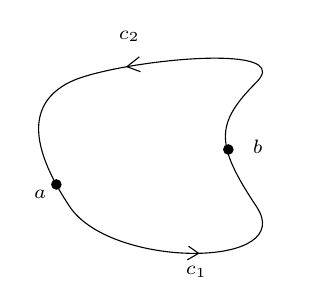
\begin{tikzpicture}[x=0.75pt,y=0.75pt,yscale=-1,xscale=1]
%uncomment if require: \path (0,300); %set diagram left start at 0, and has height of 300

%Shape: Polygon Curved [id:ds9093612224966613] 
\draw   (168.71,103) .. controls (174.05,100.33) and (184.36,97.67) .. (196.24,95.57) .. controls (228.9,89.8) and (273.38,88.33) .. (258.71,103) .. controls (238.71,123) and (238.71,133) .. (258.71,163) .. controls (268.41,177.54) and (252.27,185.03) .. (230.78,185.48) .. controls (207.93,185.96) and (179.02,178.46) .. (168.71,163) .. controls (148.71,133) and (148.71,113) .. (168.71,103) -- cycle ;
%Shape: Circle [id:dp08160237269259418] 
\draw  [fill={rgb, 255:red, 0; green, 0; blue, 0 }  ,fill opacity=1 ] (160,152.31) .. controls (160,151.06) and (161.01,150.05) .. (162.26,150.05) .. controls (163.51,150.05) and (164.52,151.06) .. (164.52,152.31) .. controls (164.52,153.56) and (163.51,154.57) .. (162.26,154.57) .. controls (161.01,154.57) and (160,153.56) .. (160,152.31) -- cycle ;
%Shape: Circle [id:dp024322200086419055] 
\draw  [fill={rgb, 255:red, 0; green, 0; blue, 0 }  ,fill opacity=1 ] (242.86,135.45) .. controls (242.86,134.2) and (243.87,133.19) .. (245.12,133.19) .. controls (246.37,133.19) and (247.38,134.2) .. (247.38,135.45) .. controls (247.38,136.7) and (246.37,137.71) .. (245.12,137.71) .. controls (243.87,137.71) and (242.86,136.7) .. (242.86,135.45) -- cycle ;
%Straight Lines [id:da10659302097889911] 
\draw    (225.94,182.05) -- (230.78,185.48) ;
%Straight Lines [id:da9833686555678408] 
\draw    (225.36,188.62) -- (230.78,185.48) ;
%Straight Lines [id:da55759753490004] 
\draw    (196.24,95.57) -- (202.22,90.83) ;
%Straight Lines [id:da9565823802538397] 
\draw    (196.24,95.57) -- (202.79,97.97) ;

% Text Node
\draw (150.29,153.75) node [anchor=north west][inner sep=0.75pt]  [font=\scriptsize]  {$a$};
% Text Node
\draw (255.71,129.6) node [anchor=north west][inner sep=0.75pt]  [font=\scriptsize]  {$b$};
% Text Node
\draw (223.43,190.46) node [anchor=north west][inner sep=0.75pt]  [font=\scriptsize]  {$c_{1}$};
% Text Node
\draw (191.14,77.03) node [anchor=north west][inner sep=0.75pt]  [font=\scriptsize]  {$c_{2}$};
\end{tikzpicture}
\end{center}

\begin{align*}
	\oint_c \vec E \cdot \text{d} \vec l &= 0\\
	\int_{a}^{b} \vec E \cdot \text{d} \vec l &+ \int_{b}^{a} \vec E \cdot \text{d} \vec l = 0 \\
	\Rightarrow \int_{a}^{b} \vec E \cdot \text{d} \vec l &= - \int_{b}^{a} \vec E \cdot \text{d} \vec l \\
	\Rightarrow \int_{a}^{b} \vec E \cdot \text{d} \vec l &= \int_{a}^{b} \vec E \cdot \text{d} \vec l
\end{align*}
\newpage

zero-potential point $\to \infty$ \\ \\
\begin{minipage}[t]{0.4\textwidth}
\vspace{0pt}
\tikzset{every picture/.style={line width=0.75pt}} %set default line width to 0.75pt     
\begin{tikzpicture}[x=0.75pt,y=0.75pt,yscale=-1,xscale=1]
%uncomment if require: \path (0,300); %set diagram left start at 0, and has height of 300

%Straight Lines [id:da7208464817729751] 
\draw  [dash pattern={on 4.5pt off 4.5pt}]  (140.17,184.69) -- (215.45,106.79) ;
\draw [shift={(216.84,105.36)}, rotate = 134.02] [color={rgb, 255:red, 0; green, 0; blue, 0 }  ][line width=0.75]    (6.56,-1.97) .. controls (4.17,-0.84) and (1.99,-0.18) .. (0,0) .. controls (1.99,0.18) and (4.17,0.84) .. (6.56,1.97)   ;
\draw [shift={(140.17,184.69)}, rotate = 314.02] [color={rgb, 255:red, 0; green, 0; blue, 0 }  ][fill={rgb, 255:red, 0; green, 0; blue, 0 }  ][line width=0.75]      (0, 0) circle [x radius= 2.01, y radius= 2.01]   ;

% Text Node
\draw (125.33,182.4) node [anchor=north west][inner sep=0.75pt]  [font=\scriptsize]  {$q$};
% Text Node
\draw (156.67,131.07) node [anchor=north west][inner sep=0.75pt]  [font=\scriptsize]  {$R$};
% Text Node
\draw (212,90.73) node [anchor=north west][inner sep=0.75pt]  [font=\scriptsize]  {$V\ =\ ?$};
\end{tikzpicture}
\end{minipage}
\begin{minipage}[t]{0.5\textwidth}
\vspace{0pt}
	\begin{align*}
		V &= - \int_{\infty}^{R} (\hat{a_R} \cdot \frac{q}{4 \pi \epsilon_0 R^2}) \cdot (\hat{a_R} \text{d} R) \\
		\Rightarrow V &= \frac{q}{4 \pi \epsilon_0 R} \quad (V)
	\end{align*}
\end{minipage}

\begin{minipage}[t]{0.4\textwidth}
\vspace{0pt}
\tikzset{every picture/.style={line width=0.75pt}} %set default line width to 0.75pt     
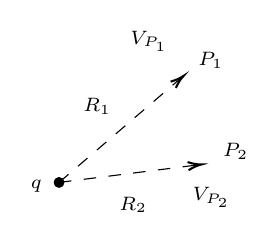
\begin{tikzpicture}[x=0.75pt,y=0.75pt,yscale=-1,xscale=1]
%uncomment if require: \path (0,300); %set diagram left start at 0, and has height of 300

%Straight Lines [id:da7208464817729751] 
\draw  [dash pattern={on 4.5pt off 4.5pt}]  (140.17,184.69) -- (198.65,134.66) ;
\draw [shift={(200.17,133.36)}, rotate = 139.45] [color={rgb, 255:red, 0; green, 0; blue, 0 }  ][line width=0.75]    (6.56,-1.97) .. controls (4.17,-0.84) and (1.99,-0.18) .. (0,0) .. controls (1.99,0.18) and (4.17,0.84) .. (6.56,1.97)   ;
\draw [shift={(140.17,184.69)}, rotate = 319.45] [color={rgb, 255:red, 0; green, 0; blue, 0 }  ][fill={rgb, 255:red, 0; green, 0; blue, 0 }  ][line width=0.75]      (0, 0) circle [x radius= 2.01, y radius= 2.01]   ;
%Straight Lines [id:da11001156713526672] 
\draw  [dash pattern={on 4.5pt off 4.5pt}]  (140.17,184.69) -- (206.85,176.27) ;
\draw [shift={(208.84,176.02)}, rotate = 172.81] [color={rgb, 255:red, 0; green, 0; blue, 0 }  ][line width=0.75]    (6.56,-1.97) .. controls (4.17,-0.84) and (1.99,-0.18) .. (0,0) .. controls (1.99,0.18) and (4.17,0.84) .. (6.56,1.97)   ;
\draw [shift={(140.17,184.69)}, rotate = 352.81] [color={rgb, 255:red, 0; green, 0; blue, 0 }  ][fill={rgb, 255:red, 0; green, 0; blue, 0 }  ][line width=0.75]      (0, 0) circle [x radius= 2.01, y radius= 2.01]   ;

% Text Node
\draw (125.33,182.4) node [anchor=north west][inner sep=0.75pt]  [font=\scriptsize]  {$q$};
% Text Node
\draw (150.67,143.07) node [anchor=north west][inner sep=0.75pt]  [font=\scriptsize]  {$R_{1}$};
% Text Node
\draw (173.33,110.4) node [anchor=north west][inner sep=0.75pt]  [font=\scriptsize]  {$V_{P_{1}}$};
% Text Node
\draw (203.33,185.73) node [anchor=north west][inner sep=0.75pt]  [font=\scriptsize]  {$V_{P_{2}}$};
% Text Node
\draw (168,190.4) node [anchor=north west][inner sep=0.75pt]  [font=\scriptsize]  {$R_{2}$};
% Text Node
\draw (206,120.73) node [anchor=north west][inner sep=0.75pt]  [font=\scriptsize]  {$P_{1}$};
% Text Node
\draw (218,164.73) node [anchor=north west][inner sep=0.75pt]  [font=\scriptsize]  {$P_{2}$};
\end{tikzpicture}
\end{minipage}
\begin{minipage}[t]{0.5\textwidth}
\vspace{0pt}
  \begin{align*}
	  V_{21} &= V_{P_2} - V_{P_1} \\
					 &= \frac{q}{4 \pi \epsilon_0} (\frac{1}{R_2} - \frac{1}{R_1})
  \end{align*}
\end{minipage}

$\vec R$ 之電位, n discrete charges $q_1, q_2 ... q_n$ at $\vec{R'_1}, \vec{R'_2} ... \vec{R'_n}$ \\
by supseposition that
$$
V = \frac{q}{4 \pi \epsilon_0} \sum_{k=1}{n} \frac{q_k}{\left| \vec R - \vec{R'_k} \right|}  \quad (V)
$$
\newpage


\textbf{Example 3-7} \\
Find out $V_P$ and $\vec E$
\begin{center}
\tikzset{every picture/.style={line width=0.75pt}} %set default line width to 0.75pt     
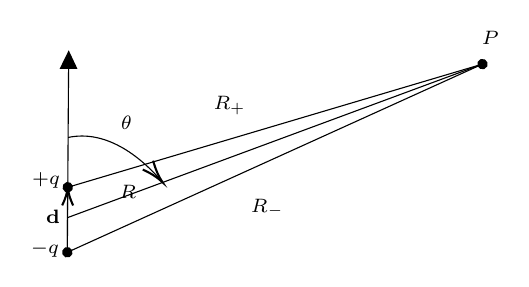
\begin{tikzpicture}[x=0.75pt,y=0.75pt,yscale=-1,xscale=1]
%uncomment if require: \path (0,300); %set diagram left start at 0, and has height of 300

%Straight Lines [id:da20418328498529592] 
\draw    (100.84,190.69) -- (100.84,174.02) -- (101.05,159.36) -- (101.21,135.36) -- (101.48,96.36) ;
\draw [shift={(101.5,93.36)}, rotate = 90.39] [fill={rgb, 255:red, 0; green, 0; blue, 0 }  ][line width=0.08]  [draw opacity=0] (8.93,-4.29) -- (0,0) -- (8.93,4.29) -- cycle    ;
%Straight Lines [id:da18738432434247987] 
\draw    (100.84,190.69) -- (300.84,100.02) ;
\draw [shift={(100.84,190.69)}, rotate = 335.61] [color={rgb, 255:red, 0; green, 0; blue, 0 }  ][fill={rgb, 255:red, 0; green, 0; blue, 0 }  ][line width=0.75]      (0, 0) circle [x radius= 2.01, y radius= 2.01]   ;
%Straight Lines [id:da17921132243484073] 
\draw    (100.84,174.02) -- (146.78,157.02) -- (300.84,100.02) ;
\draw [shift={(300.84,100.02)}, rotate = 339.7] [color={rgb, 255:red, 0; green, 0; blue, 0 }  ][fill={rgb, 255:red, 0; green, 0; blue, 0 }  ][line width=0.75]      (0, 0) circle [x radius= 2.01, y radius= 2.01]   ;
%Straight Lines [id:da9642505740759573] 
\draw    (101.05,159.36) -- (300.84,100.02) ;
\draw [shift={(101.05,159.36)}, rotate = 343.46] [color={rgb, 255:red, 0; green, 0; blue, 0 }  ][fill={rgb, 255:red, 0; green, 0; blue, 0 }  ][line width=0.75]      (0, 0) circle [x radius= 2.01, y radius= 2.01]   ;
%Straight Lines [id:da7853146965974115] 
\draw    (100.84,190.69) -- (101.04,161.36) ;
\draw [shift={(101.05,159.36)}, rotate = 90.39] [color={rgb, 255:red, 0; green, 0; blue, 0 }  ][line width=0.75]    (8.74,-2.63) .. controls (5.56,-1.12) and (2.65,-0.24) .. (0,0) .. controls (2.65,0.24) and (5.56,1.12) .. (8.74,2.63)   ;
%Curve Lines [id:da6776434012345312] 
\draw    (101.21,135.36) .. controls (119.41,131.52) and (135.5,144.26) .. (145.56,155.61) ;
\draw [shift={(146.78,157.02)}, rotate = 229.54] [color={rgb, 255:red, 0; green, 0; blue, 0 }  ][line width=0.75]    (10.93,-3.29) .. controls (6.95,-1.4) and (3.31,-0.3) .. (0,0) .. controls (3.31,0.3) and (6.95,1.4) .. (10.93,3.29)   ;

% Text Node
\draw (82.67,151.07) node [anchor=north west][inner sep=0.75pt]  [font=\scriptsize]  {$+q$};
% Text Node
\draw (82,184.07) node [anchor=north west][inner sep=0.75pt]  [font=\scriptsize]  {$-q$};
% Text Node
\draw (89.33,169) node [anchor=north west][inner sep=0.75pt]  [font=\scriptsize] [align=left] {\textbf{d}};
% Text Node
\draw (125.33,123.73) node [anchor=north west][inner sep=0.75pt]  [font=\scriptsize]  {$\theta $};
% Text Node
\draw (124.67,157.07) node [anchor=north west][inner sep=0.75pt]  [font=\scriptsize]  {$R$};
% Text Node
\draw (170,114.4) node [anchor=north west][inner sep=0.75pt]  [font=\scriptsize]  {$R_{+}$};
% Text Node
\draw (188,163.73) node [anchor=north west][inner sep=0.75pt]  [font=\scriptsize]  {$R_{-}$};
% Text Node
\draw (299.33,82.73) node [anchor=north west][inner sep=0.75pt]  [font=\scriptsize]  {$P$};
\end{tikzpicture}
\end{center}
\textit{Sol.}
\begin{align*}
	V &= \frac{q}{4 \pi \epsilon_0} (\frac{1}{R_+} - \frac{1}{R_-}) \\
	\because R &\gg d \\
	\therefore R_+ &\approx (R- \frac{d}{2} \cos \theta) \text{ and } R_- \approx (R + \frac{d}{2} \cos \theta) \\
	V &= \frac{q}{4 \pi \epsilon_0} (\frac{1}{R - \frac{d}{2} \cos \theta} - \frac{1}{R + \frac{d}{2} \cos \theta}) \\
		&= \frac{q}{ 4 \pi \epsilon_0} (\frac{d \cos \theta}{R^2 - \frac{d^2}{4} \cos^2 \theta}) \\
	\because R &\gg d \quad \therefore R^2 \gg \frac{d^2}{4} \cos^2 \theta \\
	\Rightarrow V &\simeq \frac{qd \cos \theta}{4 \pi \epsilon_0 R^2} \\
	\because \hat{a_R} \cdot \vec d &= d \cos \theta \\
	\therefore V &= \frac{q \vec d \hat{a_R}}{4 \pi \epsilon_0 R^2}
\end{align*}

Defined that $\vec P = q \vec d$ as electric dipole moment ($C \cdot m$)
$$
V = \frac{\vec P \cdot \hat{a_R}}{4 \pi \epsilon_0 R^2}
$$
For $\vec E$
\begin{align*}
	\because \vec E &= - \nabla V = -\hat{a_R} \frac{\partial V}{\partial R} - \hat{a_{\theta}} \frac{\partial V}{R \partial \theta} \\
	\therefore \vec E &= \frac{qd}{4 \pi \epsilon_0 R^3} (\hat{a_R}2\cos \theta + \hat{a_{\theta}} \sin \theta)
\end{align*}
\newpage

a continouse distribution of charge \\
a volume charge distribution
$$
V = \frac{1}{4 \pi \epsilon_0} \int_{V'} \frac{\rho_s}{R} \text{d} V' \quad (V)
$$
a surface charge distribution
$$
V = \frac{1}{4 \pi \epsilon_0} \int_{S'} \frac{\rho_s}{R} \text{d} s' \quad (V)
$$
a line charge distribution
$$
V = \frac{1}{4 \pi \epsilon_0} \int_{L'} \frac{\rho_s}{R} \text{d} l' \quad (V)
$$

Conductors in static electric field \\
Since inside a conductor $\rho_v = 0$ \\
Therefore $E = 0$

\end{document}
